
%----------------------------------------------------------------%
%----------------------------------------------------------------%

\chapter{Sex Differences in Mortality Following Hospitalization}
\label{ch:paper1}

%----------------------------------------------------------------%
%----------------------------------------------------------------%

% AUTHORS %
\textbf{Publication:}
\textsc{\underline{Andreas H\"ohn}, Lisbeth Aagaard Larsen, Daniel Christoph Schneider, 
		Rune Lindahl-Jacobsen, Roland Rau, Kaare Christensen, and Anna Oksuzyan:} 
		Sex differences in the 1-year risk of dying following all-cause and cause-specific hospital 
		admission after age 50 in comparison with a general and non-hospitalized population: A 
		register-based cohort study of the Danish population. \textbf{BMJ open} 2018;8(7),e021813. \textit{\doi{10.1136/bmjopen-2018-021813}} 

%----------------------------------------------------------------%%----------------------------------------------------------------%

\newpage

\section{Abstract}

\textbf{Objectives:} We examine the mortality of men and women within the first 
year after all-cause and cause-specific hospital admission 
to investigate whether the sex differences in mortality 
after hospitalization are higher than in the corresponding 
general and non-hospitalized population.\\
\textbf{Design:} This is a population-based, longitudinal study with 
nationwide coverage. The study population was identified 
by linking the National Patient Register with the Central 
Population Register using a 5\% random sample of the Danish 
population.\\
\textbf{Setting:} The population born between 1898 and 1961, who was alive 
and residing in Denmark after 1977, was followed up between 
1977 and 2011 with respect to hospital admissions and mortality 
while aged 50-79.\\
\textbf{Primary Outcome Measures:} The absolute sex 
differences in the 1-year risk of dying after all-cause 
and cause-specific hospital admission. The hospitalized 
population sex differentials were then compared with 
the sex differences in a general and a non-hospitalized 
population, randomly matched by age, sex and hospitalization 
status.\\
\textbf{Results:} The risk of dying was consistently higher 
for hospitalized men and women. At all ages, the absolute 
sex differences in mortality were largest in the hospitalized 
population, were smaller in the general population and were 
smallest in the non-hospitalized population. This pattern 
was consistent across all-cause admissions, and with respect 
to admissions for neoplasms, circulatory diseases and 
respiratory diseases. For all-cause hospital admissions, 
absolute sex differences in the 1-year risk of dying resulted 
in 43.8 excess male deaths per 1,000 individuals within 
the age range 50-79, while the levels were lower in the 
general and the non-hospitalized population, at levels 
of 13.5 and 6.6, respectively.\\
\textbf{Conclusions:} This study indicates a larger male 
disadvantage in mortality following hospitalization, pointing 
towards an association between the health status of a population 
and the magnitude of the female advantage in mortality.


%-------------------------------------%


\section{Strengths and Limitations of this Study}
\begin{itemize}
	\item 	This study uses high-quality Danish register data, 
			with nationwide coverage, that leave little room 
			for selection bias due to non-response or loss to 
			follow-up.
	\item 	Our findings of excess male mortality within the 
			first year after all-cause hospitalization compared 
			with their female counterparts remain robust when 
			stratifying by the main causes of admission to hospital 
			in Denmark.
	\item	Due to a lack of further medical data on the admissions, 
			including information on risk factors and severity of 
			diseases, we were not able to disentangle the potential 
			behavioral and biological mechanisms behind widening sex 
			differences after hospitalization.
\end{itemize}

%-------------------------------------%

\newpage

\section{Background}

Empirical studies have consistently reported that women have 
a mortality advantage at all ages, starting at infancy and 
extending over the entire life course.\citep{drevenstedt2008rise} 
Women have lower rates of mortality than men for nearly all 
causes of death, including most cancers,\citep{najari2013sex,
edgren2012,cook2011} respiratory diseases\citep{de2009sex,
dransfield2007gender} and accidents.\citep{waldron2005trends} 
Moreover, the female advantage in mortality persists even 
after stressful events during the life course, such as 
bereavement\citep{stroebe2007health,moon2011widowhood} or 
famines and epidemics.\citep{zarulli2018women} While the 
relative sex differences in mortality peak at around age 
25 and tend to become smaller with age,\citep{gjonca2005} 
the absolute sex differences grow almost exponentially 
between ages 40 and 90, as general levels of mortality 
increase.\citep{wisser2014sex} Thus, in recent decades, 
the largest share of the sex differences in life expectancy 
has been attributed to mortality differentials after the 
age of 50\citep{beltran2015} — when individuals start to 
accumulate diseases and disabilities, and the incidence of 
most adverse health conditions increases.\citep{christensen2009ageing}

A number of previous studies have argued that a hospital 
admission may serve as a quasi-objective indicator of health. 
An admission to the hospital may indicate the onset of a health 
decline or the manifestation of a health decline that started 
long ago that now requires extensive medical interventions.\citep{karampampa2013trends,
karampampa2014,case2005sex} The use of hospitalization as a 
proxy for health is supported by previous research findings 
showing that adults of all ages who rate their health and 
their quality of life as poor are at an increased risk of 
hospital admission.\citep{fleury2014predictors,farkas2010self,
desalvo2005predicting,kennedy2001repeated} Furthermore, 
the well-established associations between major risk factors 
and the increased risk of dying from certain causes, such 
as smoking and lung cancer, have also been found for the 
relationship between risk factors and cause-specific reasons 
of admission.\citep{hanlon2007analysis,hanlon2000link,hanlon1998hospital} 
Empirical findings have demonstrated that smoking,\citep{hanlon2007analysis} 
hazardous drinking,\citep{smyth2015alcohol} being overweight,\citep{reeves2014hospital} 
having high cholesterol levels\citep{crowe2013risk} and a 
lack of physical activity\citep{garcia2006regular} are related 
to an increased risk of hospital admission. The presence of 
multiple risk factors has been found to be especially strongly 
associated with a high risk of admission.\citep{syddall2016understanding}

Although it has been well established that women have a mortality 
advantage across all ages and all causes of death, it is not 
yet known whether this advantage changes after the manifestation 
of bad health, which we measure as a hospital admission. To answer 
this question, we estimate the absolute sex differences in the 
1-year risk of dying after all-cause and cause-specific hospital 
admission as an inpatient. We compare these absolute sex differentials 
with the corresponding differences we would have observed in 
the general and the non-hospitalized population.\\

%-------------------------------------%

\section{Methods and Materials}

\subsection{Data}

This study uses a 5\% random sample of the Danish population. 
Using the unique personal identification number that is assigned 
to all individuals residing in Denmark,\citep{thygesen2011} we 
linked records from the National Patient Register (NPR) with 
data of the Central Population Registry (CPR). The CPR, which 
covers the entire population alive and residing in Denmark since 
1968, contains information on each resident's vital status, sex 
and place and date of birth.\citep{pedersen2011} The NPR is a 
population-based register with nationwide coverage that contains 
information on all admissions to hospitals since 1977.\citep{lynge2011} 
As reports to the administration are compulsory, the NPR data 
have high levels of completeness and reliability, making these 
data an excellent tool for research.\citep{andersen1999} Whereas 
data on hospitalizations are available for the period 1977--2011, 
the vital status of individuals was traceable up to the year 
2013. In the NPR, diagnoses were classified in accordance with 
the International Classification of Diseases (ICD), 8th Revision 
until 1993 and the ICD 10th Revision starting in 1994.\citep{schmidt2014} 
We classified the causes of admission to hospital according to 
the main chapters and used broad groups to reduce the potential 
bias, which may emerge from combining two systems of classification. 
An overview of the coding is given in \hyperref[ch2:tabS1]{Supplementary Table S1} 
at the end of this paper.\\

\subsection{Study Population}

We identified all individuals who were born between 1 January 1898 
and 31 December 1961, who were alive and who resided in Denmark 
after 1968 in the 5\% random sample (n=214,613). Of those, we then 
selected all individuals who survived up to age 50 and resided in 
Denmark after 1 January 1977 (n=198,580). Out of all remaining 
individuals, 64.3\% (n=127,642) of the sample had been admitted 
to the hospital at least once between 1 January 1977 and 31 December 
2011. Hospitalization was defined as the first time an individual 
was admitted to the hospital while aged 50--79 as an inpatient, 
for at least one night and for any reason between the years 1977 
and 2011. Subsequent admissions and admissions that occurred among 
these individuals before the age of 50, after age 79 and before 1977 
-- for the same or other causes -- were not taken into account.

To examine whether the sex differences in mortality increase following 
an admission to hospital, we compared the sex differentials after 
hospitalization with the corresponding differences measured among 
two healthier references. For this purpose, two matched populations 
aged 50--79 were selected randomly from the study sample: one group 
to represent the general population, and the other group to represent 
the non-hospitalized population. Each hospitalized individual was 
matched to one individual from each reference group. The matched 
individuals forming the two reference populations had to be the same 
age (+/- 30 days), the same sex and alive on the day the corresponding 
case was hospitalized. Whereas the individuals representing the 
general population were selected irrespective of hospitalization 
status, the individuals representing the non-hospitalized population 
had not been hospitalized within a concordant year before and after 
the exact date the corresponding case was admitted to the hospital, 
irrespective of the case's cause of admission. Cases and matches were 
drawn from the same source population. We used matching with replacement 
to correct the observed distortion that a certain proportion of the 
hospitalized population would have remained without a match, which 
emerged when matching without replacement was tested. The matching 
was carried out 100 times to increase the robustness of the matching 
results, and to bypass the need to choose a single matching scenario. 
Consequently, the same person may appear more than once in each of 
the 100 matching scenarios.\\

\subsection{Patient and Public Involvement}
No patients were involved in setting the research question or the 
outcome measures, nor were they involved in developing plans for 
design or implementation of the study. No patients were asked to 
advise on interpretation or writing up of results. No patients were 
involved in the recruitment to and conduct of the study. There are 
no plans to disseminate the results of the research to study 
participants or the relevant patient community.\\

\subsection{Statistical Analysis}
The survival time of the hospitalized individuals starts immediately 
with the day of the first all-cause hospital admission after age 50, 
which was recorded in the registers. No lag time or washout period 
was used to ensure that the immediate impact of the manifestation of 
bad health on the risk of dying was captured, implying that deaths 
during the index hospital stay are included in the mortality calculations. 
Analogously, the process time of the individuals of both reference 
populations starts on the day the corresponding case was hospitalized. 
The survival status of all individuals was followed up within 1 year. 
If a person was alive by the end of the follow-up period or had migrated, 
this individual was considered as having no event. We used a generalized 
additive model (GAM) for binary data with a logit link. Unlike in 
generalized linear models, the linear predictor in the GAM is replaced 
by a sum of smoothing functions.\citep{hastie1986generalized,hastie1995generalized} 
We used penalized B-splines, so-called P-splines, as basis functions 
in the regression to smooth over age.\citep{wood2006generalized,
eilers1996flexible} We modeled the age-specific 1-year risk of dying 
separately for the men and the women of each population by single years 
of age. For the hospitalized population, we further estimated separate 
models by cause of admission to hospital to investigate whether the 
female advantage in survival following hospitalization varies across 
different causes of admission. While the data preparation and the merging 
of registries was carried out with STATA (Version 14), all statistical 
analyses were performed in R (Version 3.3.2).\\

\section{Results}
Of the 127,642 individuals who were hospitalized, 49.9\% (n=63,649) were 
men and 50.1\% (n=63,993) were women. The mean age at hospitalization was 
slightly lower among the men (61.7; SD=8.5) than among the women (62.0; 
SD=9.0). An overview on the causes of admission to hospital is provided 
in \hyperref[ch2:tab1]{Table 1} .

\begin{table}[H]
  \scriptsize
  \centering
  \caption*{\textbf{Table 1: }  Overview of causes of admission to hospital by sex}
    \begin{tabular}{lrrrr}
    \toprule
    \multicolumn{1}{c}{\textbf{Cause of Hospital}} & \multicolumn{2}{c}{\textbf{Men }} & \multicolumn{2}{c}{\textbf{Women}} \\
    \multicolumn{1}{c}{\textbf{Admission}} & \multicolumn{1}{c}{\textbf{Number}} & \multicolumn{1}{c}{\textbf{Share in \%}} & \multicolumn{1}{c}{\textbf{Number }} & \multicolumn{1}{c}{\textbf{Share in \%}} \\
    \midrule
    Infectious \& parasitic diseases & 980   & 1.54  & 1,012 & 1.58 \\
    Neoplasms & 6,625 & 10.41 & 9,310 & 14.55 \\
    Diseases of blood \& blood-forming organs & 266   & 0.42  & 401   & 0.63 \\
    Endocrine, nutritional \& metabolic diseases & 1,368 & 2.15  & 2,220 & 3.47 \\
    Mental \& behavioral disorders & 1,000 & 1.57  & 883   & 1.38 \\
    Diseases of the nervous system & 1,434 & 2.25  & 1,382 & 2.16 \\
    Diseases of the eye \& adnexa & 1,026 & 1.61  & 1,464 & 2.29 \\
    Diseases of the ear \& mastoid process & 461   & 0.72  & 496   & 0.78 \\
    Iscaemic heart diseases & 5,899 & 9.27  & 2,601 & 4.06 \\
    Cerebrovascular diseases & 2,386 & 3.75  & 1,756 & 2.74 \\
    Other circulatory diseases & 6,324 & 9.94  & 5,368 & 8.39 \\
    Respiratory Diseases & 3,785 & 5.95  & 3,233 & 5.05 \\
    Digestive diseases & 8,368 & 13.15 & 6,166 & 9.64 \\
    Diseases of the skin \& subcutaneous tissue & 786   & 1.23  & 700   & 1.09 \\
    Musculosceletal disorders & 4,737 & 7.44  & 5,858 & 9.15 \\
    Diseases of the genitourinary system & 4,680 & 7.35  & 6,968 & 10.89 \\
    Injuries, poisionings \& accidents & 6,466 & 10.16 & 7,228 & 11.29 \\
    All other diseases* & 7,058 & 11.09 & 6,947 & 10.86 \\
    \midrule
    \textbf{Total } & \textbf{63,649} & \textbf{100.00} & \textbf{63,993} & \textbf{100.00} \\
    \bottomrule
    \bottomrule
\multicolumn{5}{c}{\textit{* The largest groups among the category of all other diseases are symptoms, signs and}}\\
\multicolumn{5}{c}{\textit{abnormal clinical and laboratory findings (men: 57.57\%, women: 58.42\%) and factors}} \\
\multicolumn{5}{c}{\textit{influencing the health status and contact with health services (men: 37.47\%, women: 36.99\%) }} \\
    \end{tabular}
\label{ch2:tab1}
\end{table}%

We found the distribution of causes of hospital admission to 
be different in men and in women. In comparison with men, women were more 
likely to be hospitalized due to neoplasms, diseases of the blood and 
blood-forming organs, endocrine, nutritional and metabolic diseases, 
diseases of the eye and adnexa, musculoskeletal disorders and diseases 
of the genitourinary system. In contrast, more men were admitted due to 
ischaemic heart diseases, cerebrovascular diseases and other circulatory 
diseases, as well as due to respiratory and digestive diseases than women. 
We found only small sex differences in the distribution with respect to 
infectious and parasitic diseases, mental and behavioral disorders, diseases 
of the nervous system, diseases of the ear and mastoid process, diseases 
of the skin and subcutaneous tissue as well as injuries, poisonings and 
accidents.

An overview of the three populations is given in \hyperref[ch2:tab2]{Table 2}. While the data 
for the hospitalized population represent the exact number of observed cases, 
the numbers for the general and the non-hospitalized population refer to 
the mean of 100 matched samples. Because the matched individuals were of 
the same age and the same sex as the corresponding cases, the three populations 
had identical age structures (mean=61.9, SD=8.9) and sex ratios. We found 
that the risk of dying was highest among the men and the women of the 
hospitalized population at the level of 9.42\% (95\% CI: 9.26\% to 9.58\%). 
The risk of dying was substantially lower and at the level of 1.98\% (95\% 
CI: 1.90\% to 2.05\%) in the corresponding general population, and lowest 
among the non-hospitalized population at a level of 0.80\% (95\% CI: 0.75\% 
to 0.85\%), respectively. As shown in \hyperref[ch2:tab2]{Table 2}, men had consistently higher
mortality than women in all of the three populations. In all populations, 
we found the mortality of both sexes to increase consistently with age.

We further estimated the risk of dying and the trajectory of this risk by 
single years of age for men and women in each population and corresponding 
95\% CI using a non-parametric GAM. As shown in \hyperref[ch2:fig1]{Figure 1}, 
we found that men had consistently higher mortality than their female counterparts 
in each population, at all ages and for admissions due to all causes, 
neoplasms, circulatory and respiratory diseases. The risk of dying increased 
consistently with age among the men and the women in each population, 
and with respect to all causes of admission to hospital.

\begin{landscape}

\begin{table}[H]
  \scriptsize
  \centering
  \caption*{\textbf{Table 2: }  Number of individuals, number of deaths 
  			and the risk of dying within 1 year of follow-up by sex and 
  			age in the hospitalized, general and non-hospitalized population}
    \begin{tabular}{ccccccccc}
    \toprule
    \textbf{Age at } & \multicolumn{4}{c}{\textbf{Men}} & \multicolumn{4}{c}{\textbf{Women}} \\
    \textbf{Admission /} & \multicolumn{2}{c}{\textbf{Ind.}} & \multicolumn{2}{c}{\textbf{Deaths}} & \multicolumn{2}{c}{\textbf{Ind.}} & \multicolumn{2}{c}{\textbf{Deaths}} \\
    \textbf{of Matches} & \textbf{No.} & \textbf{Share (\%)} & \textbf{No.} & \textbf{Risk (\%)} & \textbf{No.} & \textbf{Share (\%)} & \textbf{No.} & \textbf{Risk (\%)} \\
    \midrule
          &       &       &       &       &       &       &       &  \\
          & \multicolumn{8}{c}{\textbf{Hospitalized Population}} \\
          &       &       &       &       &       &       &       &  \\
    50--54 & \multicolumn{1}{r}{18,397} & \multicolumn{1}{r}{28.90} & \multicolumn{1}{r}{906} & \multicolumn{1}{r}{4.92} & \multicolumn{1}{r}{19,569} & \multicolumn{1}{r}{30.58} & \multicolumn{1}{r}{622} & \multicolumn{1}{r}{3.18} \\
    55--59 & \multicolumn{1}{r}{12,392} & \multicolumn{1}{r}{19.47} & \multicolumn{1}{r}{898} & \multicolumn{1}{r}{7.25} & \multicolumn{1}{r}{11,432} & \multicolumn{1}{r}{17.86} & \multicolumn{1}{r}{514} & \multicolumn{1}{r}{4.50} \\
    60--64 & \multicolumn{1}{r}{10,493} & \multicolumn{1}{r}{16.49} & \multicolumn{1}{r}{1,074} & \multicolumn{1}{r}{10.24} & \multicolumn{1}{r}{9,244} & \multicolumn{1}{r}{14.45} & \multicolumn{1}{r}{655} & \multicolumn{1}{r}{7.09} \\
    65--69 & \multicolumn{1}{r}{9,030} & \multicolumn{1}{r}{14.19} & \multicolumn{1}{r}{1,320} & \multicolumn{1}{r}{14.62} & \multicolumn{1}{r}{8,508} & \multicolumn{1}{r}{13.30} & \multicolumn{1}{r}{844} & \multicolumn{1}{r}{9.92} \\
    70--74 & \multicolumn{1}{r}{7,623} & \multicolumn{1}{r}{11.98} & \multicolumn{1}{r}{1,432} & \multicolumn{1}{r}{18.79} & \multicolumn{1}{r}{7,967} & \multicolumn{1}{r}{12.45} & \multicolumn{1}{r}{1,046} & \multicolumn{1}{r}{13.13} \\
    75--79 & \multicolumn{1}{r}{5,714} & \multicolumn{1}{r}{8.98} & \multicolumn{1}{r}{1,457} & \multicolumn{1}{r}{25.50} & \multicolumn{1}{r}{7,273} & \multicolumn{1}{r}{11.37} & \multicolumn{1}{r}{1,261} & \multicolumn{1}{r}{17.34} \\
    \textbf{Total} & \multicolumn{1}{r}{\textbf{63,649}} & \multicolumn{1}{r}{\textbf{100.00}} & \multicolumn{1}{r}{\textbf{7,087}} & \multicolumn{1}{r}{\textbf{11.13}} & \multicolumn{1}{r}{\textbf{63,993}} & \multicolumn{1}{r}{\textbf{100.00}} & \multicolumn{1}{r}{\textbf{4,942}} & \multicolumn{1}{r}{\textbf{7.72}} \\
          &       &       &       &       &       &       &       &  \\
          & \multicolumn{8}{c}{\textbf{General Population*}} \\
          &       &       &       &       &       &       &       &  \\
    50--54 & \multicolumn{1}{r}{18,400} & \multicolumn{1}{r}{28.91} & \multicolumn{1}{r}{124} & \multicolumn{1}{r}{0.68} & \multicolumn{1}{r}{19,558} & \multicolumn{1}{r}{30.56} & \multicolumn{1}{r}{88} & \multicolumn{1}{r}{0.45} \\
    55--59 & \multicolumn{1}{r}{12,394} & \multicolumn{1}{r}{19.47} & \multicolumn{1}{r}{145} & \multicolumn{1}{r}{1.17} & \multicolumn{1}{r}{11,452} & \multicolumn{1}{r}{17.90} & \multicolumn{1}{r}{80} & \multicolumn{1}{r}{0.70} \\
    60--64 & \multicolumn{1}{r}{10,486} & \multicolumn{1}{r}{16.47} & \multicolumn{1}{r}{195} & \multicolumn{1}{r}{1.86} & \multicolumn{1}{r}{9,231} & \multicolumn{1}{r}{14.43} & \multicolumn{1}{r}{100} & \multicolumn{1}{r}{1.08} \\
    65--69 & \multicolumn{1}{r}{9,042} & \multicolumn{1}{r}{14.21} & \multicolumn{1}{r}{268} & \multicolumn{1}{r}{2.97} & \multicolumn{1}{r}{8,520} & \multicolumn{1}{r}{13.31} & \multicolumn{1}{r}{153} & \multicolumn{1}{r}{1.80} \\
    70--74 & \multicolumn{1}{r}{7,612} & \multicolumn{1}{r}{11.96} & \multicolumn{1}{r}{369} & \multicolumn{1}{r}{4.85} & \multicolumn{1}{r}{7,961} & \multicolumn{1}{r}{12.44} & \multicolumn{1}{r}{218} & \multicolumn{1}{r}{2.74} \\
    75--79 & \multicolumn{1}{r}{5,714} & \multicolumn{1}{r}{8.98} & \multicolumn{1}{r}{449} & \multicolumn{1}{r}{7.85} & \multicolumn{1}{r}{7,270} & \multicolumn{1}{r}{11.36} & \multicolumn{1}{r}{334} & \multicolumn{1}{r}{4.60} \\
    \textbf{Total} & \multicolumn{1}{r}{\textbf{63,649}} & \multicolumn{1}{r}{\textbf{100.00}} & \multicolumn{1}{r}{\textbf{1,551}} & \multicolumn{1}{r}{\textbf{2.44}} & \multicolumn{1}{r}{\textbf{63,993}} & \multicolumn{1}{r}{\textbf{100.00}} & \multicolumn{1}{r}{\textbf{974}} & \multicolumn{1}{r}{\textbf{1.52}} \\
          &       &       &       &       &       &       &       &  \\
          & \multicolumn{8}{c}{\textbf{Non-Hospitalized Population*}} \\
          &       &       &       &       &       &       &       &  \\
    50--54 & \multicolumn{1}{r}{18,400} & \multicolumn{1}{r}{28.91} & \multicolumn{1}{r}{57} & \multicolumn{1}{r}{0.31} & \multicolumn{1}{r}{19,558} & \multicolumn{1}{r}{30.56} & \multicolumn{1}{r}{27} & \multicolumn{1}{r}{0.14} \\
    55--59 & \multicolumn{1}{r}{12,393} & \multicolumn{1}{r}{19.47} & \multicolumn{1}{r}{53} & \multicolumn{1}{r}{0.43} & \multicolumn{1}{r}{11,452} & \multicolumn{1}{r}{17.90} & \multicolumn{1}{r}{21} & \multicolumn{1}{r}{0.18} \\
    60--64 & \multicolumn{1}{r}{10,488} & \multicolumn{1}{r}{16.48} & \multicolumn{1}{r}{76} & \multicolumn{1}{r}{0.72} & \multicolumn{1}{r}{9,232} & \multicolumn{1}{r}{14.43} & \multicolumn{1}{r}{32} & \multicolumn{1}{r}{0.34} \\
    65--69 & \multicolumn{1}{r}{9,042} & \multicolumn{1}{r}{14.21} & \multicolumn{1}{r}{108} & \multicolumn{1}{r}{1.20} & \multicolumn{1}{r}{8,521} & \multicolumn{1}{r}{13.32} & \multicolumn{1}{r}{52} & \multicolumn{1}{r}{0.61} \\
    70--74 & \multicolumn{1}{r}{7,612} & \multicolumn{1}{r}{11.96} & \multicolumn{1}{r}{150} & \multicolumn{1}{r}{1.97} & \multicolumn{1}{r}{7,958} & \multicolumn{1}{r}{12.44} & \multicolumn{1}{r}{83} & \multicolumn{1}{r}{1.05} \\
    75--79 & \multicolumn{1}{r}{5,713} & \multicolumn{1}{r}{8.98} & \multicolumn{1}{r}{150} & \multicolumn{1}{r}{2.63} & \multicolumn{1}{r}{7,271} & \multicolumn{1}{r}{11.36} & \multicolumn{1}{r}{154} & \multicolumn{1}{r}{2.12} \\
    \textbf{Total} & \multicolumn{1}{r}{\textbf{63,649}} & \multicolumn{1}{r}{\textbf{100.00}} & \multicolumn{1}{r}{\textbf{656}} & \multicolumn{1}{r}{\textbf{1.03}} & \multicolumn{1}{r}{\textbf{63,993}} & \multicolumn{1}{r}{\textbf{100.00}} & \multicolumn{1}{r}{\textbf{369}} & \multicolumn{1}{r}{\textbf{0.58}} \\
    \midrule
    \midrule
    \multicolumn{9}{c}{\textit{* the number of deaths and the risk of dying refer to the average of 100 matching results}} \\
    \end{tabular}%
\label{ch2:tab2}
\end{table}%

\end{landscape}


	%------------------%
	\begin{figure}[H]
		\centering
		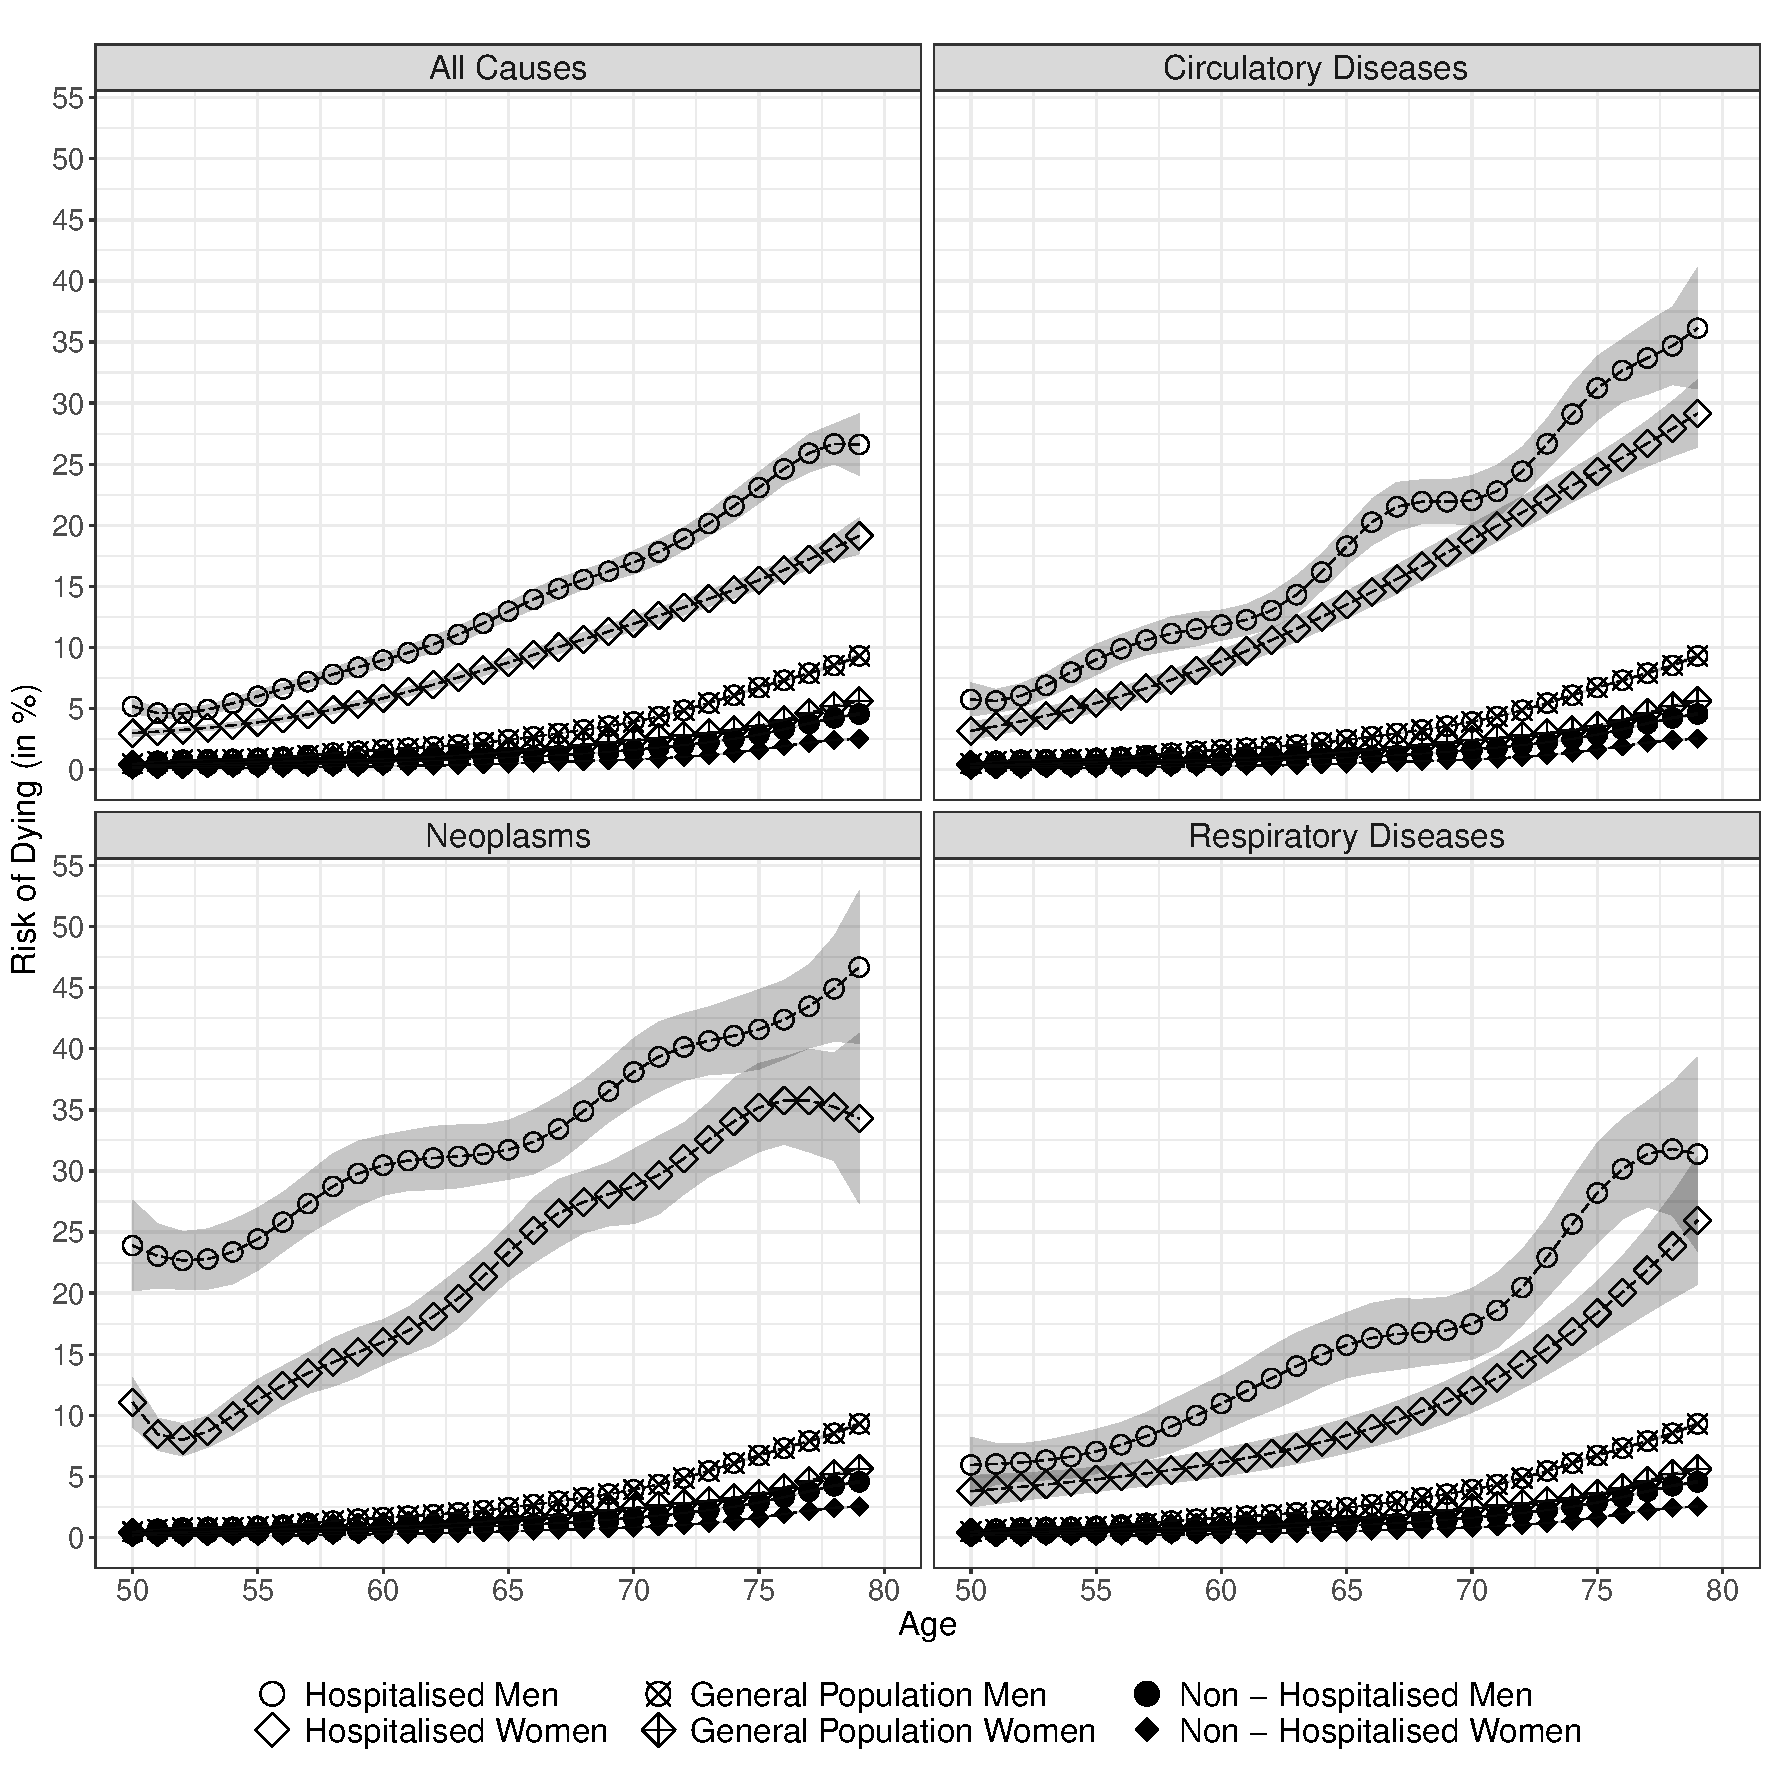
\includegraphics[scale=0.425]{Paper_1/Paper1_Fig_1}
		\caption*{	\textbf{Figure 1: } Estimated age trajectories in the risk of dying 
					within 1 year of follow-up by cause of admission to hospital}
	\label{ch2:fig1}
	\end{figure}
	%--------------------%


At the age of 50, the 1-year risk of dying for all-cause admissions in 
the hospitalized population was 5.17\% (95\% CI: 4.60\% to 5.73\%) for 
men and 2.97\% (95\% CI: 2.66\% to 3.29\%) for women. With age, the risk 
of dying increased and reached a level of 26.61\% (95\% CI: 24.08\% to 
29.13\%) and 19.12\% (95\% CI: 17.65\% to 20.60\%) among 79-year-old men 
and women of the hospitalized population, for men and women respectively.

We found the absolute increase in mortality with age to be smaller in 
the general population than in the hospitalized population. Starting 
with levels of 0.47\% (95\% CI: 0.46\% to 0.49\%) among men and 0.39\% 
(95\% CI: 0.38\% to 0.41\%) among women at age 50, the risk of dying 
was 9.30\% (95\% CI: 9.12\% to 9.47\%) and 5.61\% (95\% CI: 5.49\% to 
5.73\%) at the age of 79 in the general population, respectively.

We found the non-hospitalized population to have the lowest absolute 
increase in mortality with age: at age 50, the risk of dying was 0.25\% 
(95\% CI: 0.24\% to 0.26\%) for men and 0.12\% (95\% CI: 0.11\% to 0.13\%) 
for women, and it increased to 4.54\% (95\% CI: 4.42\% to 4.67\%) and 
2.52\% (95\% CI: 2.43\% to 2.60\%) at age 79, respectively.

In a next step, we calculated the absolute sex differences in the 
1-year risk of dying and the the male excess mortality per 1,000 persons. 
\hyperref[ch2:fig2]{Figure 2} shows the age trajectory of the male excess mortality in each 
of the three populations and by cause of admission to hospital. At all 
ages and regarding admissions for all causes, neoplasms, circulatory 
and respiratory diseases, the absolute sex differences were largest in 
the hospitalized population, were smaller in the general population, 
and were smallest in the non-hospitalized population. At age 50 and 
for all-cause admissions, the sex differences in survival resulted in 
22.0 excess male deaths per 1,000 individuals in the hospitalized 
population, while there were 0.8 excess male deaths in the general 
population, and 1.3 excess male deaths in the non-hospitalized population.

Within the observed age range, the excess male mortality increased 
almost steadily among all three populations, resulting at levels 
of 42.0, 9.8 and 4.8 excess male deaths per 1,000 individuals at 
age 65, and levels of 74.8, 36.9 and 20.3 at age 79, respectively. 
For all-cause hospital admissions, the larger absolute sex differences 
in the 1-year risk of dying resulted, on average, in 43.8 excess male 
deaths per 1000 individuals within the age range 50-79, while the 
levels were lower in the general and the non-hospitalized population, 
at levels of 13.5 and 6.6, respectively. While the male excess 
mortality after all-cause hospital admission increases steadily with 
age, the pattern differs when broken down by specific causes of admission. 
Whereas for admissions due to circulatory and respiratory diseases 
the male excess mortality shows a similar increasing pattern, the male 
excess mortality is highest at younger ages for admissions due to 
neoplasms and decreases with age.\\


	%--------------------%
	% FIGURE 2: ABS DIFF %
	\begin{figure}[H]
		\centering
		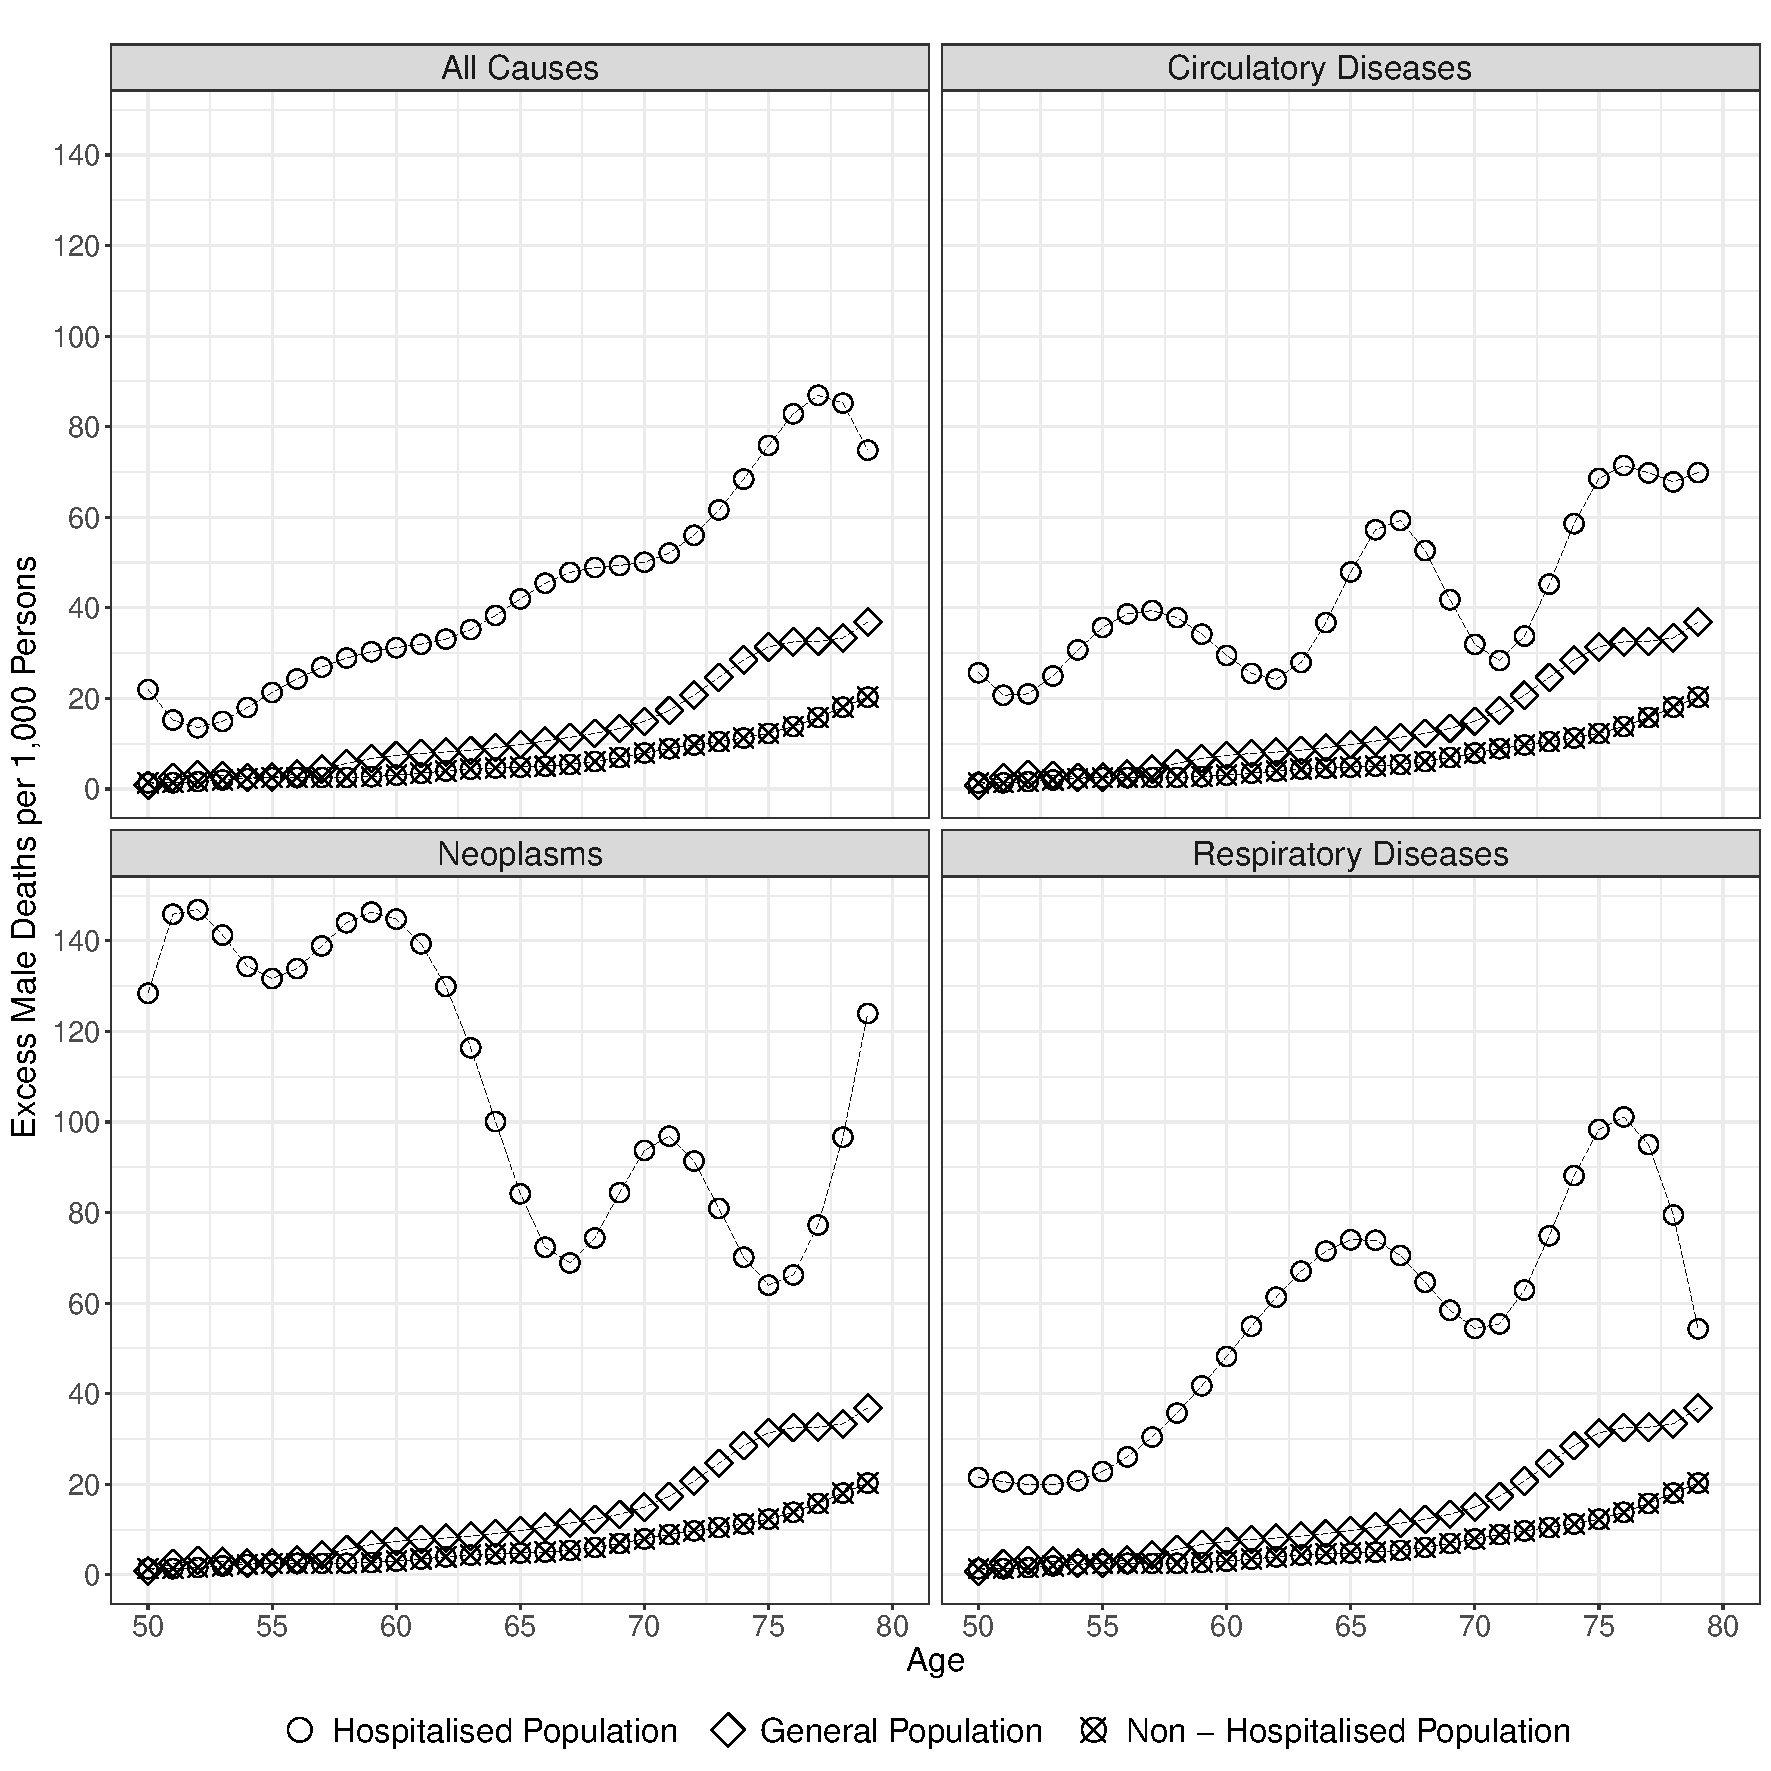
\includegraphics[scale=0.425]{Paper_1/Paper1_Fig_2}
		\caption*{\textbf{Figure 2 } Male excess mortality within 1 year of follow-up by 
				 cause of admission to hospital.}
	\label{ch2:fig2}	
	\end{figure}
	%--------------------%	

	
%-------------------------------------%


\section{Discussion}

\subsection{Principle Findings}
In this study, we investigated how women's mortality advantage changes 
after the manifestation of an adverse health condition, which we measured 
as a hospital admission. We estimated the absolute sex differences in 
the 1-year risk of dying after an all-cause and cause-specific hospitalization 
among the population aged 50--79, and compared these patterns with those 
observed in a matched general and non-hospitalized population. As expected, 
women had consistently lower mortality than men in all three populations. 
In addition, we found that the absolute sex differences in mortality were 
highest for the hospitalized population, were lower in the general population, 
and were lowest in the non-hospitalized population. The excess male mortality 
always remained larger in the hospitalized population when differentiating 
by cause of admission to hospital.\\

\subsection{Strengths and Weaknesses of the Study}
In this study, we used Danish register data, which provide nationwide 
coverage and are representative of the total Danish population. In contrast 
to longitudinal survey data, these register data suffer less in terms of 
non-response and loss to follow-up; issues that could have biased the 
analyses and led to skewed results.\citep{oksuzyan2008} Another strength 
is that we were able to examine mortality for the overarching all-cause 
hospital admissions as well as the mortality patterns for cause-specific 
hospital admissions. This allowed us to establish if the larger male excess 
mortality following hospitalization was present across different causes 
of hospital admission, representing admissions for the major causes of 
death in Denmark. Similar patterns of sex differences in all-cause and 
cause-specific admissions suggest that the larger sex differences in 
mortality after hospital admission cannot be fully explained by differences 
in the distribution of causes of admission among men and women. In order 
to minimize the bias due to changes in ICD coding over the study period, 
we used broad categories to group causes of hospital admission.

We calculated the absolute sex differences in the 1-year risk of dying 
after an admission to hospital. This allowed us to directly compare the 
male excess mortality in the hospitalized, the general, and the non-hospitalized 
population. It has been shown that different conclusions about health 
inequalities might be the result of the effect measure used. This has 
been shown in relation to mortality differences between socioeconomic 
groups, across countries, over time,\citep{moser2007comparing} and in 
respect to sex differences.\citep{wisser2014sex,harper2005methods} We 
therefore replicated the analysis using risk ratios (see \hyperref[ch2:figS1]{Supplementary Figure S1} 
at the end of the paper). Using risk ratios leads to a different 
interpretation, that the sex differences were lowest among the hospitalized 
individuals and highest for the non-hospitalized population where the 
overall risk of mortality was lowest. Both, absolute and relative measures 
are context dependent and their use needs to be justified.\citep{moser2007comparing} 
Problems surrounding the interpretation of risk ratios often appear 
when populations under investigation differ in their overall risks 
of mortality.\citep{wisser2014sex} In our case, the discrepancy between 
absolute and relative measures is driven by the fact that the three 
populations differ significantly in their initial levels of mortality. 
As we are interested in quantifying the burden of the male excess 
mortality across the three populations, an absolute measure appears 
to be most suitable as it takes into account the underlying risks of 
mortality.\citep{tramer2005number}

Our study does not address the underlying reasons for the greater excess 
male mortality in the 1-year period after admission to hospital. The 
register data did not allow us to examine the severity of the underlying 
causes of hospital admission or to control for differences in health 
behaviors. Furthermore, the study design did not allow us to examine the 
question of whether the observed gaps in survival after hospital admission 
changed over time or across cohorts. This issue may be particularly relevant 
for Denmark where the sex differentials in mortality are known to have 
been affected by a stagnation of female life expectancy during the 1977--1995 
period, which was a consequence of smoking among women born between the 
two world wars.\citep{jacobsen2016,lindahl2016did,jacobsen2008sex} The 
increased prevalence of smoking among Danish women, when compared with 
countries where the prevalence of female smokers remained low throughout 
the 20th century, may have an impact on our findings in two ways. First, 
by leading to higher levels of mortality among women of all three populations. 
Second, by leading to higher rates of admissions for smoking-related 
diseases among women. Likely, the male excess mortality would have been 
higher in all three populations in the absence of higher smoking rates 
among Danish women. The data do not allow us to quantify the impact of 
the Danish smoking phenomenon on our findings. All in all, this demonstrates 
that factors which determine the distribution of causes of admission to 
hospital and the levels of disease-specific mortality after hospitalization 
within a population are complex. Both factors may be influenced by changes 
in the organization and the performance of the healthcare system, including 
shifts in the admission strategies and the quality of medical treatment; 
or they could depend on a range of demographic characteristics, such as 
the prevalence of diseases or the distribution of risk factors in a 
population.\citep{hanlon2007analysis} 

It is important to highlight that our analysis compares men and women of 
the same age and does not control for the health status of individuals. 
However, we recognize that men tend to develop adverse health conditions 
at earlier ages than women,\citep{hubbard2011frailty,eskes2007women} and 
that studies on strokes and myocardial infarctions have shown that, on 
average, men are 8 years younger than women at the onset of these 
conditions.\citep{zhang2012age,berger2009sex,appelros2010review,appelros2009sex}

To gain a deeper understanding of the sex differences in mortality after 
hospital admission, future research should aim to identify the underlying 
reasons for these differences, and investigate how these sex disparities 
have developed over time, by cohort, and how they vary by socioeconomic 
status. Also, the length of follow-up we used needs to be taken into 
account. It could be that the increased level of mortality during the 
first year after admission is temporary, and that the duration of the 
follow-up period has an impact on the mortality levels of the hospitalized 
men and women due to selective mortality and cure. As we wanted to 
capture the immediate mortality development following hospital admission, 
we decided to use a relatively short follow-up period of 1-year length.

\subsection{Interpretation and Implications in Light of Previous Findings}
The existing literature focusing on the female mortality advantage has 
pointed towards the effects, and the interactions, of biological, behavioral 
and social factors.\citep{oksuzyan2008} The most widely cited biological 
factors are hormonal, based on the observation that the female hormone 
oestrogen has favorable effects on serum lipid levels, as well as 
vasoprotective and immune-enhancing effects, and genetic, based on the 
assumption that women's second X chromosome helps to ameliorate the harmful 
effects of gene mutations on the X chromosome.\citep{seifarth2012sex,bouman2005sex,
stindl2004,christensen2001x} Moreover, women may have stronger immune 
systems than men, which could help women to recover more quickly,\citep{oertelt2012influence} 
and may play a fundamental role in women's better survival of harsh 
conditions, including famines and epidemics.\citep{zarulli2018women} 
In addition to these biological factors, researchers have attributed 
a substantial part of the male disadvantage in mortality to behavioral and social 
factors.\citep{rieker2005rethinking} For example, it has been argued 
that men have higher rates than women of smoking, excessive drinking, 
drug use and violence.\citep{rogers2010social} In addition to this, 
a large body of previous research, including research for Denmark, 
has shown that men tend to seek medical help later than women, which 
can lead to delays in diagnosis and treatment.\citep{farrimond2012beyond,
chan2010gender,juel2008men,noone2008men,adeyemi2007men,smith2006we,smith2005patients} 
Previous studies have shown that men who are hospitalized tend to 
have conditions that are more severe, and diseases are at more advanced 
stages than those of the women who are hospitalized. However, the reasons 
for this pattern have not yet been fully understood.\citep{simmonds2014understanding}

In Denmark, hospital care is financed through taxes, and is thus available 
to all residents, regardless of their sex and socioeconomic characteristics.\citep{olesen2009delay} 
Although our results may have been affected by changes in policies related 
to hospital admission, treatment and discharge, it is likely that such 
changes would have affected men and women in similar ways. Although access 
to healthcare services is free and universal in Denmark, individuals may 
encounter hurdles in accessing healthcare services for a variety of reasons, 
including social, economic, demographic and geographic factors.\citep{starfield2012clinical} 
In Denmark, general practitioners (GPs) typically serve not just as 
gatekeepers for the use of secondary healthcare but also as care providers 
who can help patients avoid or postpone an admission to the hospital. For 
example, GPs assist patients in monitoring their health and in preventing 
the progress of many chronic conditions through regular medical check-ups, 
health consultations, the prescription of medications and other preventive 
measures.\citep{gervas2008clinical} It is possible that the higher excess 
mortality after hospital admission among men, found in our study, may be 
partially explained by sex differences in health awareness and help-seeking 
long before an adverse health condition becomes visible. Thus, the female 
advantage in survival after hospital admission is likely to be due to 
multiple factors, including biological advantages underpinned by sex differences 
in health behaviors. Our findings point towards the importance of further 
research on the possibilities of an efficient primary healthcare system, 
as well as individuals' awareness of diseases, risk factors and compliance 
with preventive measures to reduce the male excess mortality following the 
manifestation of bad health.\\

\subsection{Conclusion}
In this study, we found that the risk of dying was highest for the hospitalized 
men and women in the 1-year period after admission to hospital, was lower among 
their counterparts in the general population and was lowest among those 
individuals who were not admitted to the hospital. We found the male excess 
mortality to be larger after the manifestation of bad health, which we measured 
as a hospital admission. Our findings point towards an association between the 
health status of a population and the magnitude of the absolute female advantage 
in mortality.\\


%-------------------------------------%
%-------------------------------------%


\newpage


\section{Supplementary Material}


\subsection{Supplementary Figures}

	%------------------%
	% FORECAST I %
	\begin{figure}[H]
		\centering
		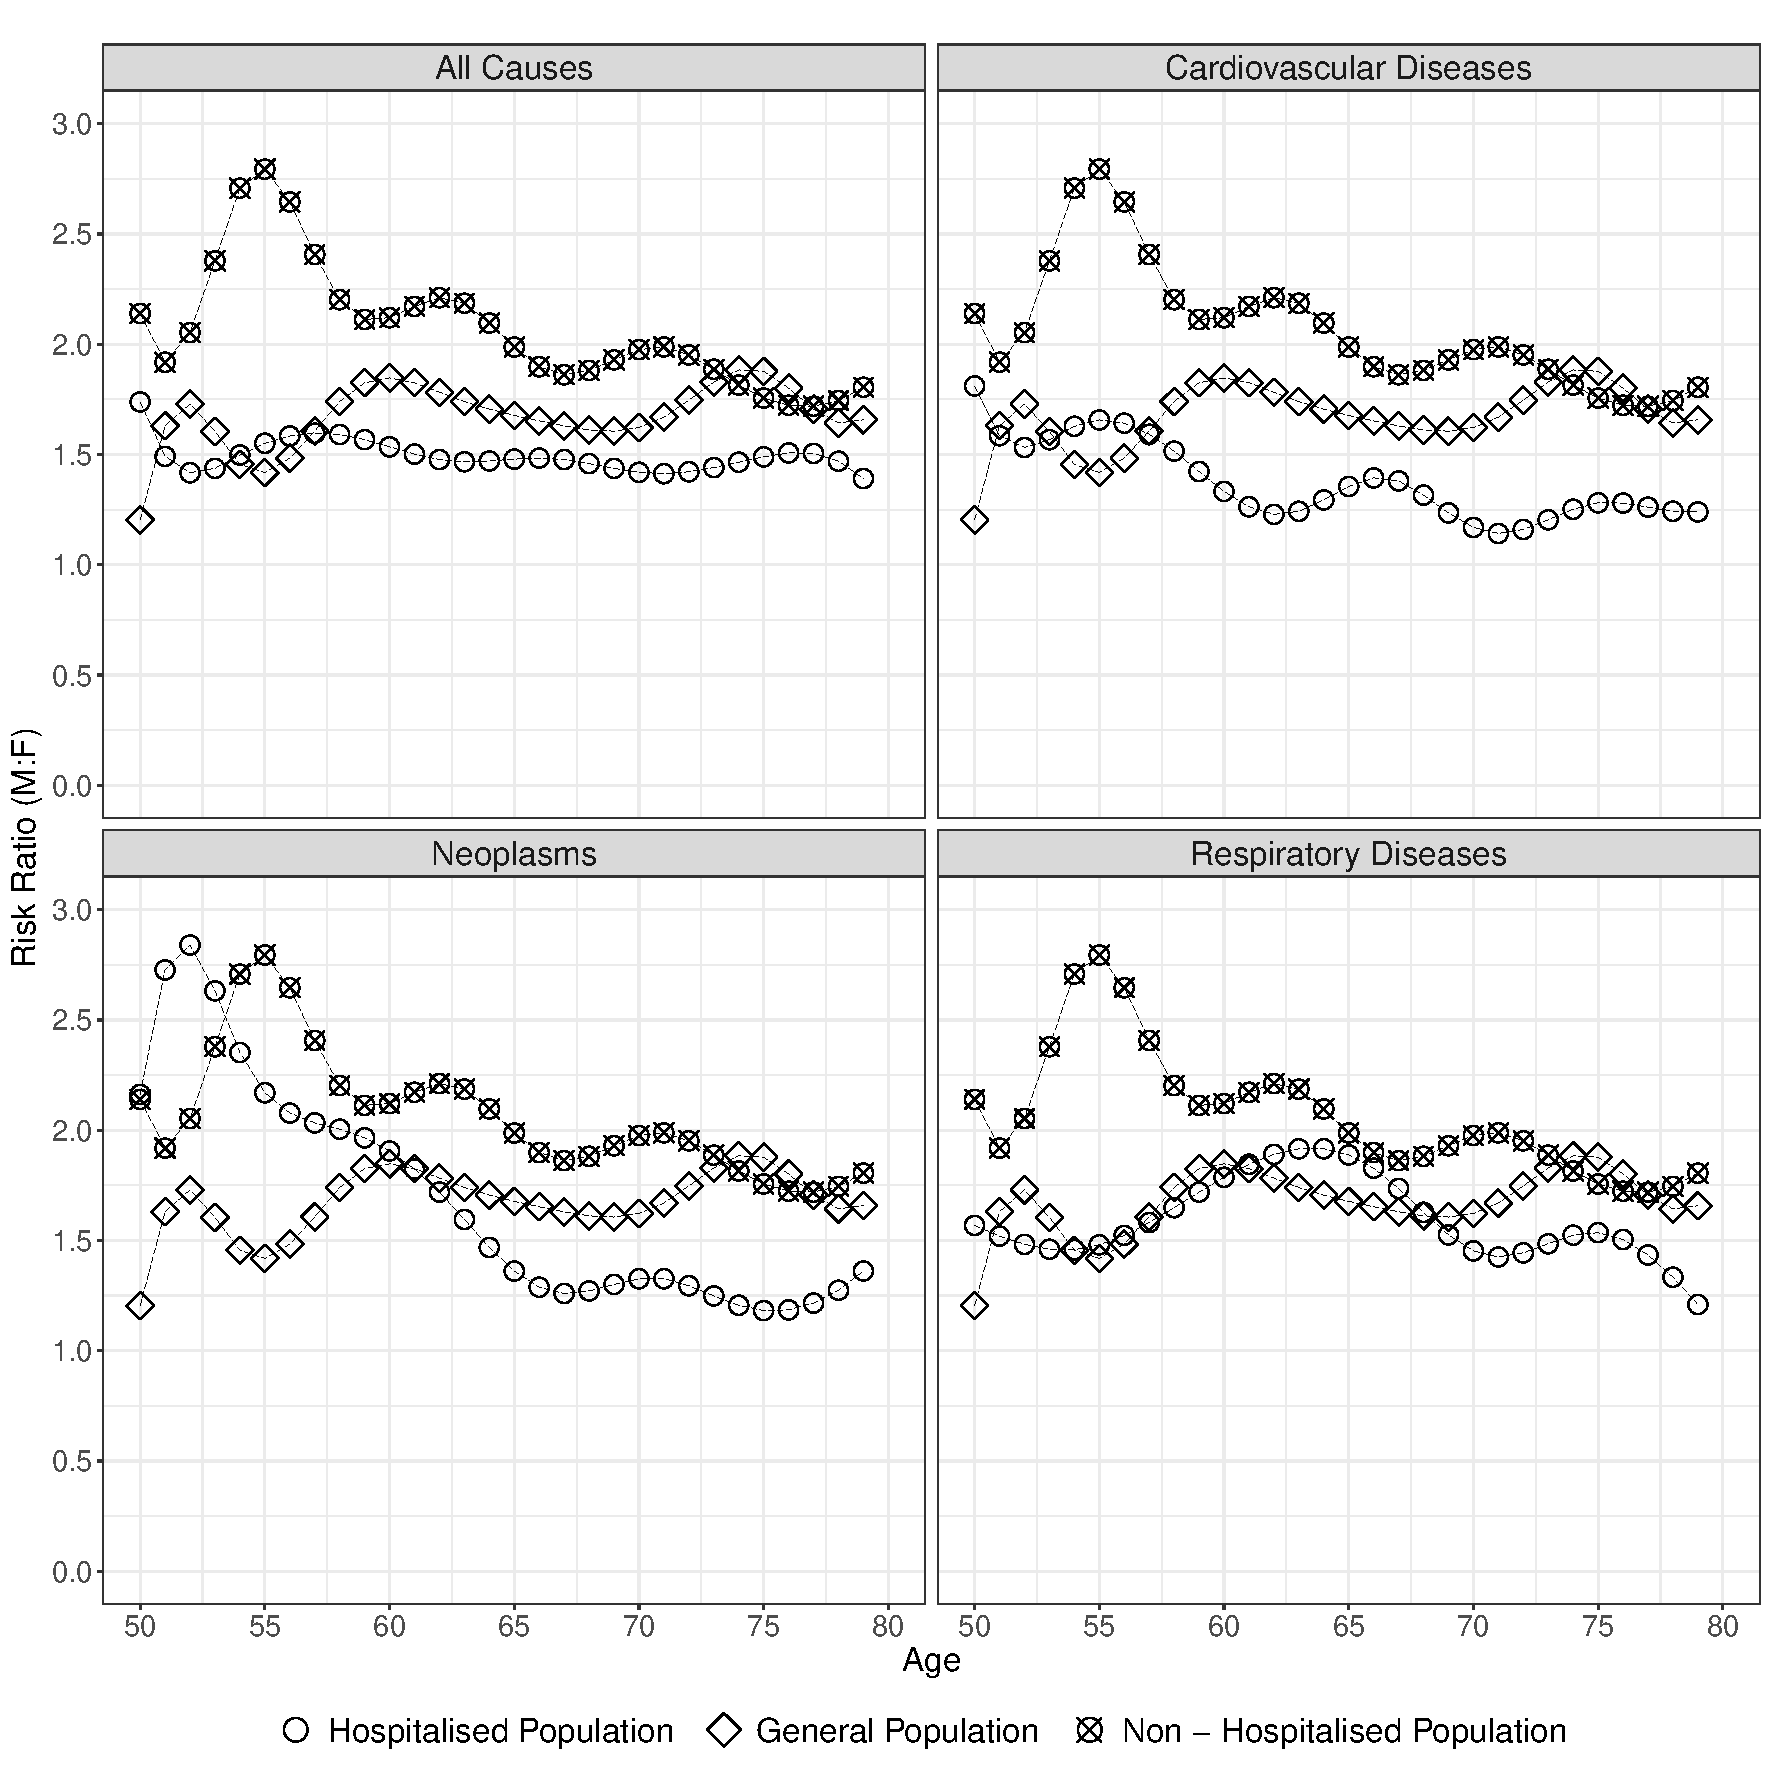
\includegraphics[scale=0.425]{Paper_1/Paper1_SuppFig_1S}
		\caption*{\textbf{Supplementary Figure S1:} Relative sex differences in the 1-year risk of dying.}
	\label{ch2:figS1}
	\end{figure}
	%--------------------%


%-------------------------------------%
%-------------------------------------%

\newpage

\subsection{Supplementary Tables}

\begin{landscape}

\begin{table}[htbp]
  \centering
  \caption*{\textbf{Supplementary Table S1:} Classification of causes of hospital admission.}
    \begin{tabular}{lcc}
    \toprule
    \textbf{Cause of Hospital Admission } & \textbf{ICD-8} & \textbf{ICD-10} \\
    \midrule
    Infectious \& parasitic diseases & 000 - 136 & A00 - B99 \\
    Neoplasms & 140 - 239 & C00 - D48 \\
    Diseases of the blood \& blood-forming organs & 280 - 289 & D50 - D89 \\
    Endocrine, nutritional \& metabolic diseases & 240 - 279 & E00 - E90 \\
    Mental \& behavioral disorders & 290 - 315 & F00 - F99 \\
    Diseases of the nervous system & 320 - 358 & G00 - G99 \\
    Diseases of the eye \& adnexa & 360 - 379 & H00 - H59 \\
    Diseases of the ear \& mastoid process & 380 - 389 & H60 - H95 \\
    Iscaemic heart diseases* & 410 - 414 & I20 - I25 \\
    Cerebrovascular diseases* & 430 - 438 & I60 - I69 \\
    Other circulatory diseases* & remaining 390 - 458 & remaining I00 - I99 \\
    Respiratory Diseases & 460 - 519 & J00 - J99 \\
    Digestive diseases & 520 - 577 & K00 - K93 \\
    Diseases of the skin \& subcutaneous tissue & 680 - 709 & L00 - L99 \\
    Musculosceletal disorders & 710 - 738 & M00 - M99 \\
    Diseases of the genitourinary system & 580 - 629 & N00 - N99 \\
    Injuries, poisionings \& accidents & 800 - 999 & S00 - T98 \& V01-Y98 \\
    All other diseases & - all other - & - all other - \\
    \bottomrule
    \bottomrule
	\multicolumn{3}{c}{\textit{* the three causes were further grouped and referred to as circulatory diseases}} \\
    \end{tabular}%
\label{ch2:tabS1}
\end{table}%

\end{landscape}



